\documentclass[tikz]{standalone}
\usepackage{tikz}
\usepackage[AutoFakeBold=true,AutoFakeSlant=true]{xeCJK}
\usepackage[zihao=-4,UTF8,heading=true]{ctex}
\usepackage[simplified]{pgf-umlcd}
\usetikzlibrary{positioning} %不加方向运算可能出错
\usetikzlibrary{arrows.meta} %箭头
\usetikzlibrary{calc}
\usetikzlibrary{fit}

\setCJKmainfont{微软雅黑}
\begin{document}
	\thispagestyle{empty}
    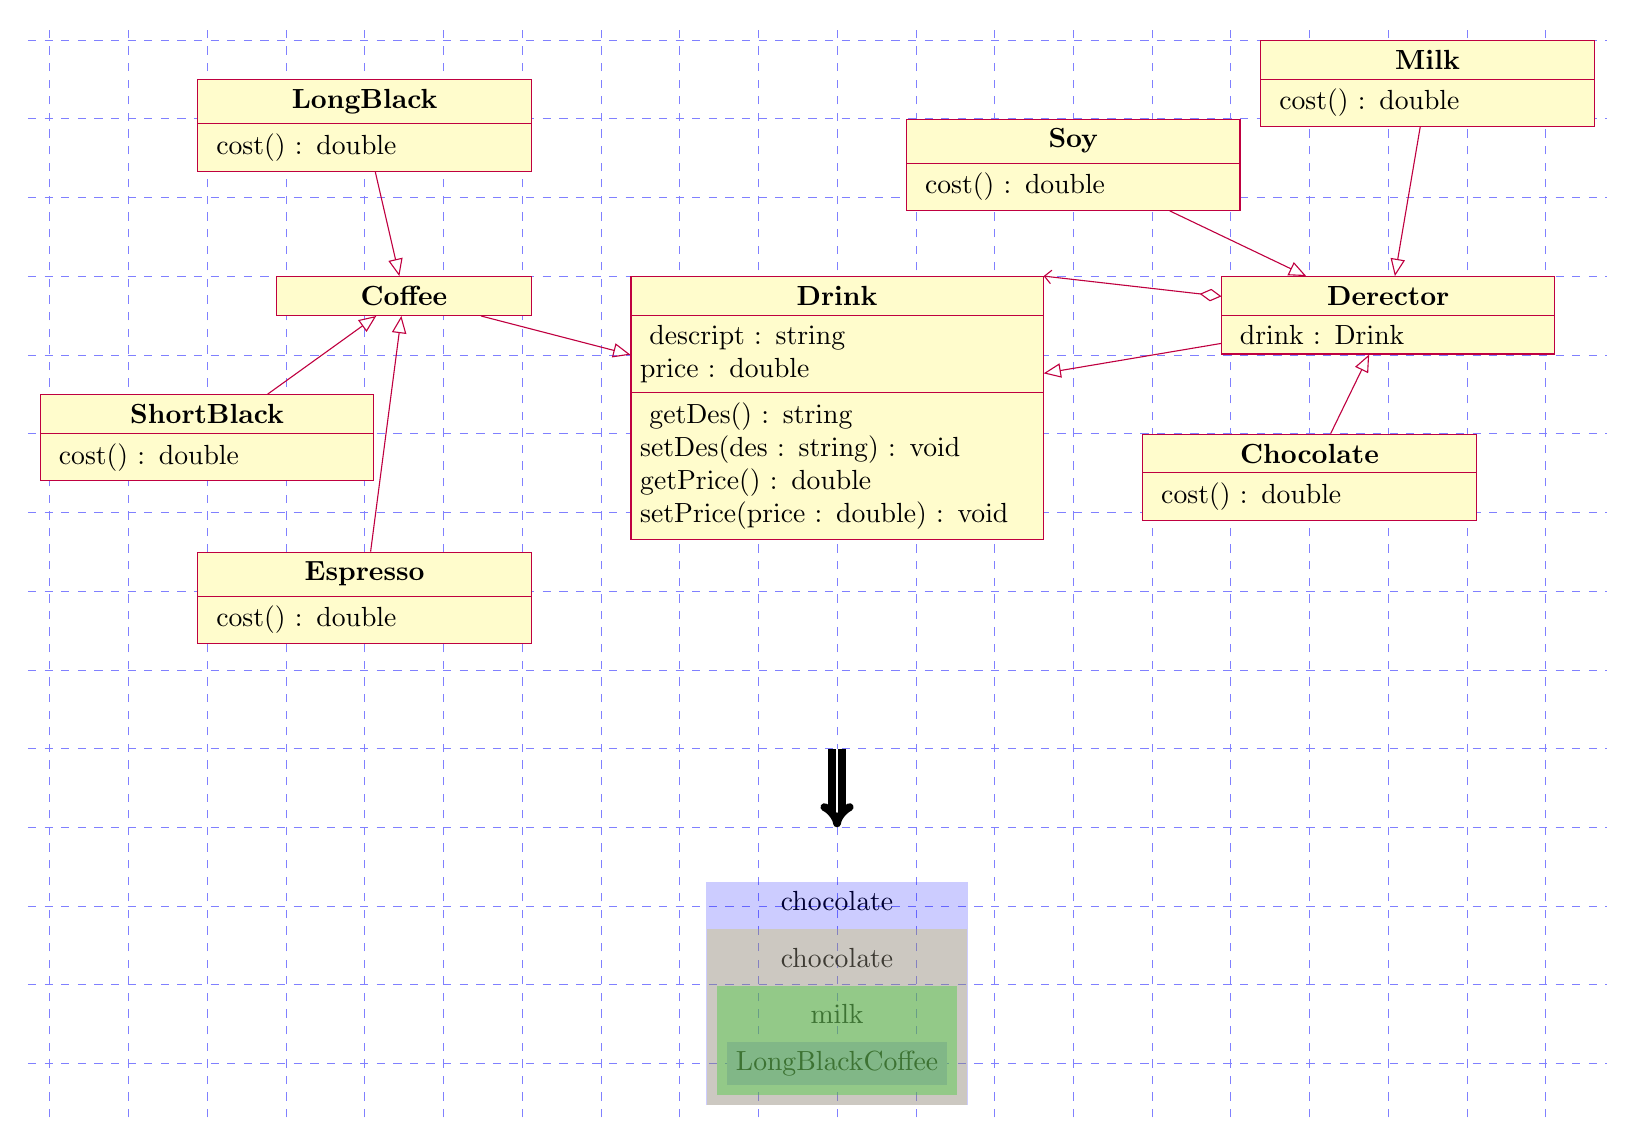
\begin{tikzpicture}[show background grid]
        \begin{class}[]{Drink}{0, 0}
            \attribute{ descript : string }
            \attribute{ price : double}
            \operation{ getDes() : string}
            \operation{ setDes(des : string) : void}
            \operation{ getPrice() : double}
            \operation{ setPrice(price : double) : void}
        \end{class}
        
        \begin{class}[text width=3cm]{Coffee}{-5.5, -0}
            \inherit{Drink}
        \end{class}
        

        \begin{class}[text width=4cm]{Derector}{7, 0}
            \inherit{Drink}
            \attribute{ drink : Drink}
        \end{class}
        \aggregation{Derector}{}{}{$(Drink.north east)$}
        
        \begin{class}[text width=4cm]{Espresso}{-6, -3.5}
            \operation{ cost() : double}
            \inherit{Coffee}
        \end{class}
        \begin{class}[text width=4cm]{ShortBlack}{-8, -1.5}
            \operation{ cost() : double}
            \inherit{Coffee}
        \end{class}
        \begin{class}[text width=4cm]{LongBlack}{-6, 2.5}
            \operation{ cost() : double}
            \inherit{Coffee}
        \end{class}

        \begin{class}[text width=4cm]{Milk}{ 7.5, 3}
            \operation{ cost() : double}
            \inherit{Derector}
        \end{class}
        \begin{class}[text width=4cm]{Chocolate}{ 6, -2}
            \operation{ cost() : double}
            \inherit{Derector}
        \end{class}
        \begin{class}[text width=4cm]{Soy}{ 3, 2}
            \operation{ cost() : double}
            \inherit{Derector}
        \end{class}
        
        \draw[-Implies, double,line width=0.1cm, name=change] (0, -6) -- (0,-7);
        

        \node[fill=blue!20, name=lbc] at (0,-10) {LongBlackCoffee};
        \node[above=0.1cm of lbc.north, name=milk] {milk};
        \node[ fit=(lbc) (milk), fill= green, name=mlbc, fill opacity=0.4] {};

        \node[name=cho1,above=0.1cm of mlbc] {chocolate};
        \node[ fit=(mlbc) (cho1), fill=yellow, name=cmlbc, fill opacity=0.3] {};
        \node[name=cho2,above=0.1cm of cmlbc] {chocolate};
        \node[ fit=(cmlbc) (cho2), fill=blue, fill opacity=0.2, name=ccmlbc, inner sep = 0.1pt] {};
    \end{tikzpicture}

        
        
\end{document}